%!TeX root = ../../Tesi.tex
Ora presentiamo un esempio di risoluzione di un sistema di equazioni lineari del tipo $A\mathbf{x}=\mathbf{b}$ mediante la funzione
\lstinline{jacobi} discussa nel paragrafo \ref{par:algoritmoJacobi}. \newline
Tutto il codice proposto di seguito \`e stato eseguito su un portatile HP Pavilion 15-eg2016nl con processore Intel\textsuperscript{\textregistered} Core\textsuperscript{\texttrademark} i7-1255U\footnote{Intel Core \`e un marchio registrato da Intel Corporation o da societ\`a da essa controllate.} e \qty{16}{\giga\byte} di memoria centrale.
\subsection{Presentazione del problema}
Consideriamo come matrice dei coefficienti $A$ la matrice derivante dalla discretizzazione dell'equazione di Poisson\footnote{
    Nonostante questo risultato del matematico francese Sim\'eon-Denis Poisson (1781-1840) sia di fondamentale importanza in meccanica,
    elettrostatica e termotecnica, non \`e nostra intenzione descrivere il problema dal punto di vista matematico.} su un
dominio quadrato $\Omega=[0, 1]\times[0, 1]$ mediante il metodo alle differenze finite.
Tale matrice viene generata ricorrendo alla funzione predefinita \lstinline{gallery}, che propone una famiglia di matrici di test per gli algoritmi sviluppati in MATLAB.
\begin{matlabcode}
    clear
    m = 385;
    n = m^2;
    A = gallery('poisson', m);
    fprintf(['\nDimensione matrice dei coefficienti A: '...
             '%u x %u \n\n'],n,n);
    b = sum(A,2);
    x = ones(n,1);
\end{matlabcode}
\begin{matlaboutput}
    Dimensione matrice dei coefficienti A: 148225 x 148225
\end{matlaboutput}
Dall'ordine della matrice $A$, notiamo che il sistema lineare considerato si presenta come un ottimo rappresentante
di un problema \textit{compute-intensive} di grandi dimensioni; fortunatamente, \lstinline{gallery} memorizza la matrice $A$ in
forma sparsa, consentendo un notevole risparmio di spazio in memoria centrale.\newline
Per costruzione, $A$ \`e una matrice a dominanza diagonale stretta per righe, propriet\`a che la rende una candidata
perfetta all'applicazione del metodo di Jacobi, come abbiamo gi\`a avuto l'occasione di sottolineare nel Teorema
\ref{teo:convergenzaDominanzaDiagonaleStretta}.

Scegliendo come vettore dei termini noti
\begin{equation*}
    \mathbf{b} = \sum_ {A_{i} \in J} A_{i},
\end{equation*}
dove $J = \{A_{1}, A_{2},\dots,A_{n}\}$ denota l'insieme delle colonne della matrice $A$, possiamo dimostrare che la soluzione $\mathbf{x}=\{{x}_{i}\}$ 
del sistema sia
\begin{equation*}
    \mathbf{x} = (1, 1, ..., 1)^\top,
\end{equation*}
essendo $\mathbf{b}$ combinazione lineare (con coefficienti pari a $\num{1}$) delle colonne $A_{i}$.
\subsection{Risoluzione con il metodo di Jacobi classico}
Dapprima, risolviamo il sistema $A\mathbf{x}=\mathbf{b}$ mediante la funzione \lstinline{jacobi} nella sua configurazione di default:
il massimo numero di iterazioni \lstinline{maxit} \`e fissato a $\num{100}$, mentre l'accuratezza della soluzione del problema \lstinline{tol} \`e pari a ${10}^{-6}$.\newline
Successivamente, calcoliamo l'errore assoluto alla $k$-esima iterazione sulla base della \eqref{eq:errorePassoK}
\begin{equation*}
\norm{\mathbf{e}^{(k)}} = \norm{\mathbf{x} - \mathbf{x}^{(k)}}.
\end{equation*}
\begin{matlabcode}
    [xJM1,flagJM1,relresJM1,iterJM1,resvecJM1] = jacobi(A,b);
    errJM1 = abs(x - xJM1);
\end{matlabcode}
\begin{matlaboutput}
    jacobi si è fermato all'iterazione numero 100 senza
    raggiungere la tolleranza desiderata 1e-06 poiché il
    numero massimo di iterazioni (100) è stato raggiunto.
    L'ultima iterazione presenta residuo relativo 
    pari a 0.028.
\end{matlaboutput}
L'errore assoluto risulta elevato dal momento che il metodo di Jacobi ha raggiunto il numero massimo di iterazioni e ha interrotto la sua esecuzione.

La funzione \lstinline{jacobi} restituisce in output \lstinline{resvec}, il vettore residuo del sistema a ogni iterazione; l'evoluzione del
residuo relativo nel corso dell'esecuzione, proposto in figura \ref{fig:evoluzioneResiduoRelativo}, pu\`o indicarci il numero di iterazioni necessarie
per il raggiungimento di una soluzione accettabile.\newline
Come secondo tentativo, eseguiamo nuovamente il metodo di Jacobi, specificando un valore di \lstinline{maxit} sufficientemente elevato per garantire la 
convergenza dell'algoritmo.
\begin{matlabcode}
    maxit = 3e5;
    tJM2 = tic;
    [xJM2,flagJM2,relresJM2,iterJM2,resvecJM2] = jacobi(A,b,
                                                 [],maxit);
    tJM2 = toc(tJM2);
    errJM2 = abs(x - xJM2);
    relresvecJM = resvecJM2./resvecJM2(1);
\end{matlabcode}
\begin{matlaboutput}
    jacobi ha raggiunto la convergenza all'iterazione 210137
    determinando una soluzione approssimata avente residuo
    relativo pari a 1e-06.

    ans =

    1.0000    1.0000    1.0000    1.0000    1.0000    ...
\end{matlaboutput}
\begin{matlaboutput}
Tempo di esecuzione per il metodo di Jacobi: 437.693564 sec.
\end{matlaboutput}
Impiegando la configurazione personalizzata, il metodo di Jacobi converge e la soluzione calcolata presenta un errore assoluto sensibilmente minore, come 
mostrato dal confronto in figura \ref{fig:confrontoErroriAssoluti}.

Il tempo di esecuzione sperimentato, pari a circa $\num{8}$ minuti per un problema di dimensioni non strabilianti, rappresenta un segnale chiaro 
dell'intensit\`a computazionale del metodo e giustifica il ricorso agli strumenti del calcolo parallelo per ottenere un miglioramento prestazionale.
\begin{figure}[!htbp]
    \centering
    \begin{subfigure}{0.6\textwidth}
        \centering
        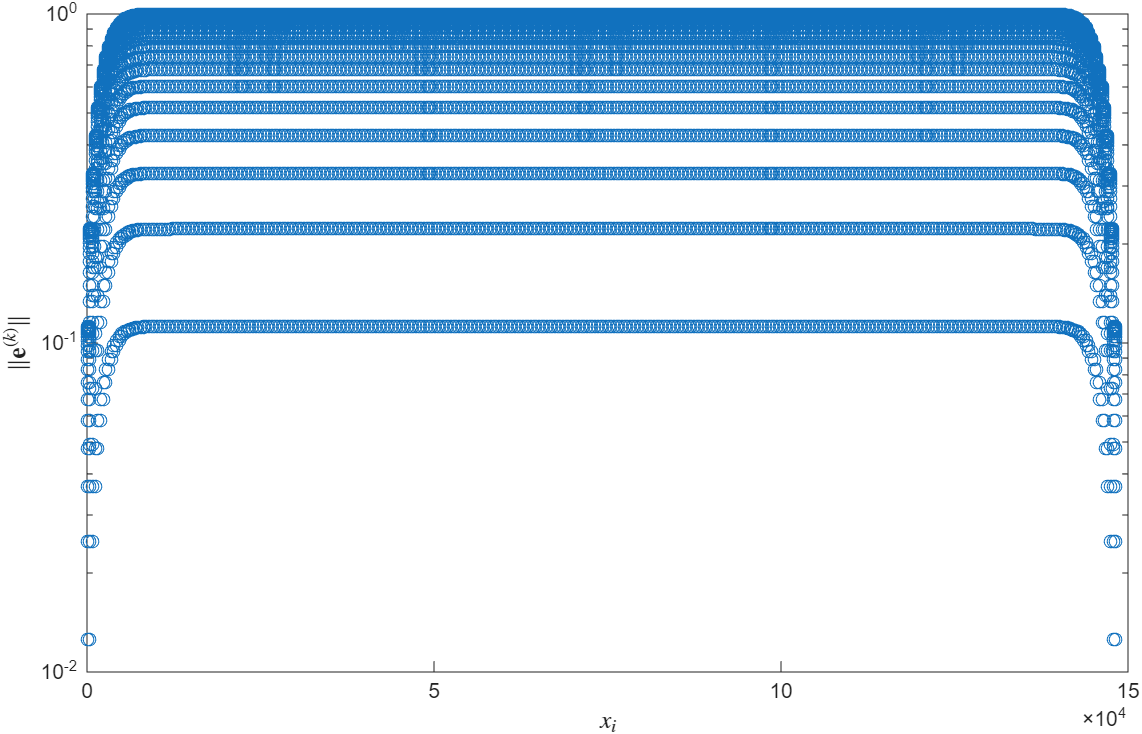
\includegraphics[width=\linewidth]{../Risorse/Capitolo 3/erroreAssolutoJacobi1.png}
        \caption{Rappresentazione dell'errore assoluto $\norm{\mathbf{e}^{(k)}}$.}
        \label{fig:erroreAssolutoJacobi1}
    \end{subfigure}

    \vspace{1.5em}

    \begin{subfigure}{0.6\textwidth}
        \centering
        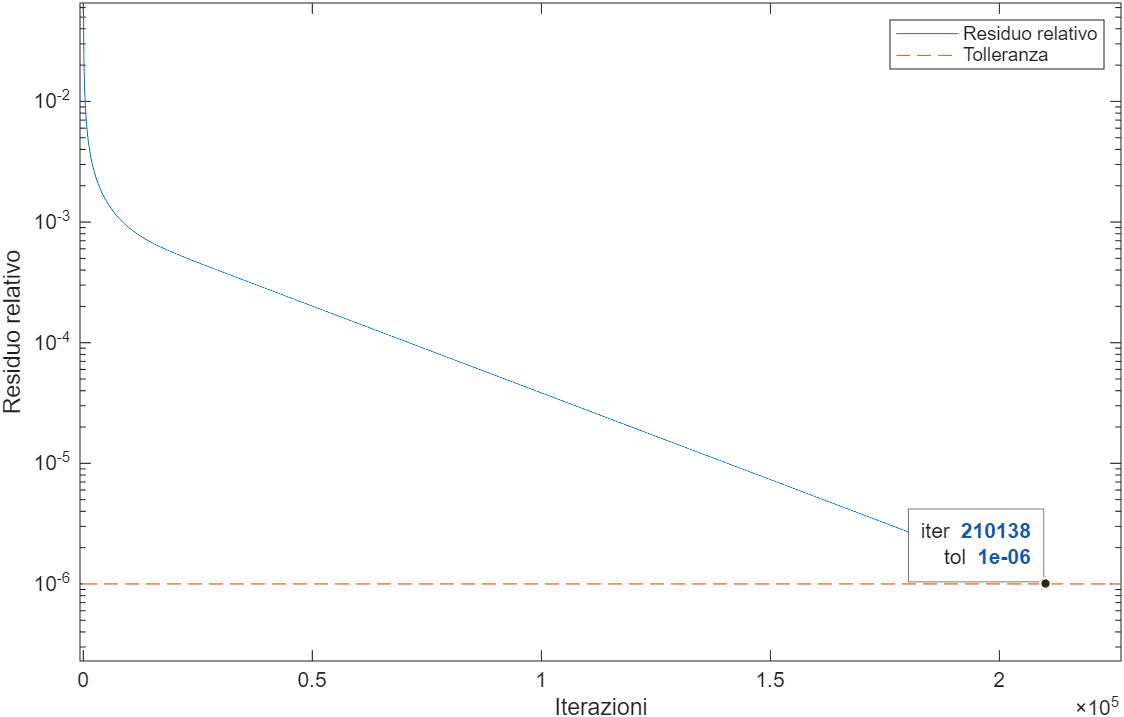
\includegraphics[width=\linewidth]{../Risorse/Capitolo 3/evoluzioneResiduoRelativo.png}
        \caption{Andamento del residuo relativo rispetto alle iterazioni completate.}
        \label{fig:evoluzioneResiduoRelativo}
    \end{subfigure}

    \vspace{1.5em}

     \begin{subfigure}{0.6\textwidth}
        \centering
        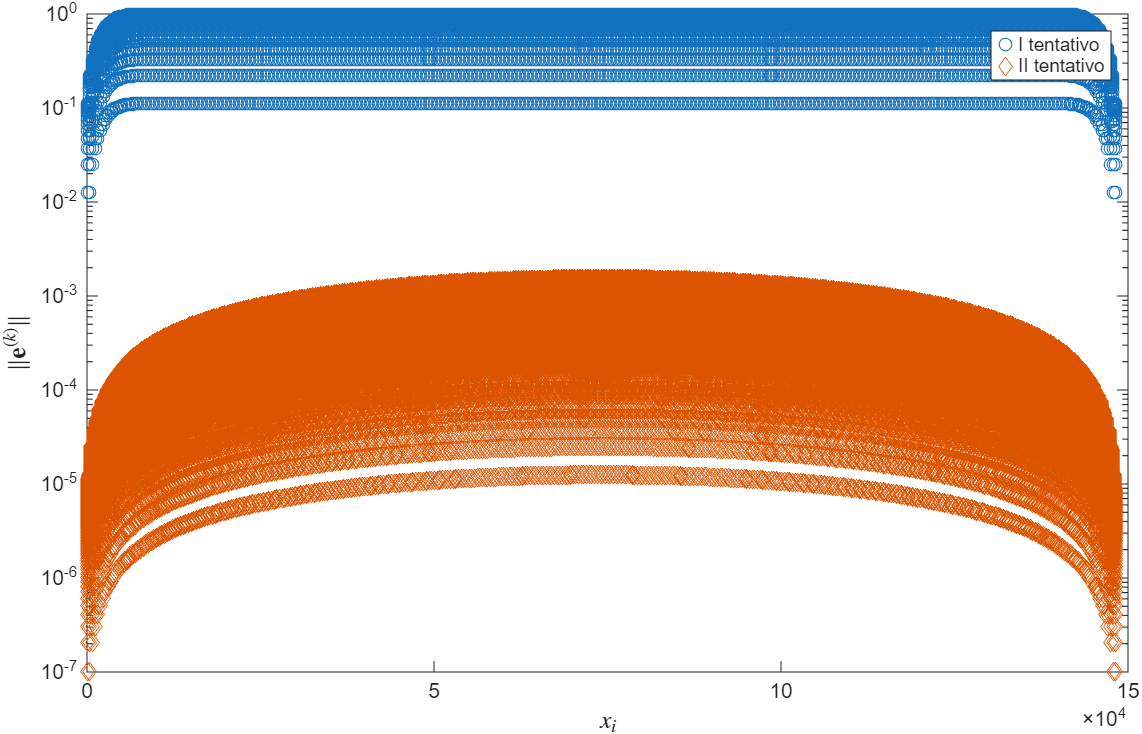
\includegraphics[width=\linewidth]{../Risorse/Capitolo 3/confrontoErroriAssoluti.png}
        \caption{Confronto degli errori assoluti tra i due tentativi di esecuzione.}
        \label{fig:confrontoErroriAssoluti}
    \end{subfigure}
    \caption{Rappresentazione dei risultati riguardanti la convergenza del metodo di Jacobi applicato al problema del paragrafo \ref{par:applicazioneMetodoJacobi}.\newline
    Quando era necessario per migliorare la leggibilit\`a del grafico, abbiamo adottato una scala logaritmica sugli assi coordinati.}
    \label{fig:gruppoImmaginiAnalisiPrestazionale}
\end{figure}
\subsection{Risoluzione con il metodo di Jacobi per \textit{array} distribuiti}
Generando la matrice $A$ come un \textit{array} distribuito, possiamo trarre vantaggio dall'esecuzione parallela della funzione \lstinline{jacobi} da parte 
di un insieme di \textit{worker} su un \textit{cluster} di elaboratori.

Questo approccio alternativo risulta vantaggioso non esclusivamente a causa dello \textit{speedup} portato dalla parallelizzazione, ma anche perch\`e 
la memorizzazione distribuita degli \textit{array} rende possibile la risoluzione di problemi in cui la matrice dei coefficienti ha dimensioni 
tali da non poter essere interamente contenuta nella memoria centrale di un singolo calcolatore.\newline
In realt\`a, l'incremento di velocit\`a viene limitato dagli \textit{overhead} di comunicazione e di sincronizzazione tra le unit\`a di lavoro, che diventano un collo di bottiglia per le \textit{performance} ogniqualvolta la dimensione del \textit{parpool} sia inadeguata rispetto all'ordine di grandezza del problema.

La generazione dei dati e la risoluzione del sistema lineare risultante sono analoghi al caso seriale, eccetto per la creazione esplicita di array 
distribuiti mediante la funzione \lstinline{distributed}.\newline
Dal momento che la funzione \lstinline{sum} pu\`o operare su un input distribuito, \lstinline{b} \`e automaticamente un \textit{array} distribuito, essendo 
calcolato a partire dalle colonne di \lstinline{A}.
\begin{matlabcode}
A = distributed((gallery('poisson', m)));
b = sum(A,2);
x = ones(m,1,'distributed');
[xJM3,flagJM3,relresJM3,iterJM3,resvecJM3] = jacobi(A,b,[],maxit);
\end{matlabcode}
\begin{matlaboutput}
    jacobi ha raggiunto la convergenza all'iterazione 210137
    determinando una soluzione approssimata avente residuo
    relativo pari a 1e-06.

    ans =

    1.0000    1.0000    1.0000    1.0000    1.0000    ...
\end{matlaboutput}
